\documentclass[11pt, letterpaper]{article}
\usepackage[utf8]{inputenc}
\usepackage{graphics}
\usepackage{graphicx}
\usepackage[francais]{babel}
\usepackage[T1]{fontenc} 
\usepackage[top=3cm, bottom=3cm, left=2cm, right=2cm]{geometry}
\usepackage{float}
\usepackage{url}
\usepackage{fancyhdr}
\usepackage[official]{eurosym}

\newcommand{\hmark}{\rule{\linewidth}{0.5mm}}

\begin{document}
\pagestyle{fancy}

\renewcommand{\headrulewidth}{1pt}
\rhead{}

\begin{titlepage}

\centering
\begin{figure}[t]
\begin{center}

\includegraphics[scale = 0.2]{upmc.png}
\end{center}
\end{figure}

\begin{center}
\par\vspace {2.5cm}
{\Huge\textbf{Rapport final : Hanabi\\*[0.25cm]}}   
\par\vspace {2cm}
{\Large\textbf{Université Pierre et Marie Curie\\ Projet ANDROIDE\\
               2015-2016}}                   
\par\vspace {2cm}
{\Large{Antunes Costa Gonçalves Daniel}}\\
{\Large{Assmann Catalina}}\\ 
{\Large{Hubert Cédric}}\\ 
{\Large{Wolfrom Matthieu}}\\
\end{center}

\end{titlepage}

\newpage

\tableofcontents

\newpage
\pagenumbering{arabic}

\section{Présentation du projet}

\subsection{Contexte}

\noindent 
Ce projet se déroule dans le contexte de l'UE Projet de première année de Master ANDROIDE de l'UPMC. Nous sommes un groupe de quatre étudiants qui doit mener à terme un projet proposé par leurs encadrants. Ce projet repose sur l'utilisation d'une intelligence artificielle qui exploite la logique épistèmique afin d'appliquer la meilleure stratégie possible pour le jeu Hanabi.

\subsection{Présentation du jeu Hanabi}

\noindent
Hanabi est un jeu de cartes coopératif composé d'un ensemble de cartes et de jetons. Les cartes représentent des feux d'artifice et les joueurs doivent collaborer afin de composer cinq feux d'artifice de couleur différente. On dispose au début de la partie de 8 jetons <<indice>> qui représentent le nombre d'indices auquel on a encore le droit, ainsi que 3 jetons <<éclair>> qui représentent le nombre d'erreur que l'on peut faire avant de perdre la partie. Les jetons sont retournés lorsqu'un indice est donné ou une erreur commise. Un jeton d'indice peut être remis sur son côté initial lorsqu'on défausse une carte.\\

\noindent
Personne ne connaît ses propres cartes, mais chacun voit les cartes des autres. En utilisant des indices et les cartes visibles, les joueurs doivent essayer de poser les feux d'artifice en suites croissantes de cartes de même couleur.\\

\noindent
Le score final est la somme des valeurs des dernières cartes posées pour chaque couleur.\\

\noindent
Pour réussir ce défi, chaque joueur peut à son tour soit donner un indice à un autre joueur, soit défausser une carte, soit jouer une carte.\\

\noindent
Un indice consiste à indiquer quelles cartes sont d'une certaine couleur ou d'une certaine valeur. Un indice négatif peut aussi être donné, indiquant qu'un joueur ne possède aucune carte d'une certaine couleur ou valeur. à chaque indice, un jeton <<indice>> est utilisé et donc retourné. Si le joueur choisit de défausser une carte, il regagne un jeton <<indice>>. Par contre, quand un joueur tente sa chance et joue une carte, il est possible que la carte ne complète pas la suite de sa couleur de feu d'artifice, dans ce cas un jeton <<éclair>> est retourné. Une fois que trois jetons éclairs sont retournés, le jeu est fini et les joueurs ont perdu.\\

\subsection{Objectifs}

\noindent
L'objectif de ce projet est de créer un logiciel qui permet à un joueur humain de jouer à Hanabi avec une ou plusieurs intelligences artificielles (maximum quatre). Nous allons proposer plusieurs modes de jeu :\\

\noindent
 Facile :

\begin{itemize}

 \item[$\bullet$] Avec ou sans jetons
 \item[$\bullet$] Avec toutes les cartes visibles\\
 
\end{itemize}

\noindent
 Normal :

\begin{itemize}

 \item[$\bullet$] Avec deux à cinq joueurs, toujours au plus un joueur humain. Pour une partie entre 2 ou 3 joueurs, chaque joueur a 5 cartes. Pour plus de joueurs, chaque joueur a 4 cartes.
 \item[$\bullet$] Avec toutes les IAs partageant la même stratégie ou avec des stratégies différentes.\\
 L'utilisateur peut y jouer via une interface graphique qui lui permettra de voir les cartes de son équipe, mais pas les siennes. \\
 
\end{itemize}

\noindent
Il y aura des options pour sauvegarder sa partie et la continuer ultérieurement. 

\subsection{Description de l'existant}

\noindent
Le logiciel est réalisé avec le langage Java, et est déployable sous les principales plateformes le supportant. Nous l'avons choisi car c'est un langage orienté objet et donc bien organisé avec des classes bien reparties. \\

\noindent
L'interface graphique est réalisée en Java Swing.\\

\noindent
Nous avons également choisi Java, car c'est un langage que les quatre membres de l'équipe ont déjà manipulé.\\

\section {Expression des besoins}

\subsection{Besoins fonctionnels}

\noindent
Le logiciel doit permettre à l'utilisateur de jouer une partie du jeu Hanabi avec d'autres joueurs artificiels. Pour ceci, nous avons besoin de créer les fonctionnalités suivantes : 

\subsubsection{L'interface Graphique}

\paragraph{Un menu d'accueil}

\begin{enumerate}

 \item  {Les règles du jeu}
 
  L'utilisateur peut cliquer sur ce bouton pour qu'on lui affiche les règles du jeu.\\


 \item  {Continuer une ancienne partie}
 
 L'utilisateur peut cliquer sur ce bouton pour qu'on lui affiche les parties sauvegardées et en choisir une pour la continuer.\\

 
 \item  {Commencer une nouvelle partie}

En cliquant sur ce bouton, le joueur voit une fenêtre qui lui affichera un formulaire avec plusieurs modes de jeu : \\

 \begin{itemize}
    \item[$\bullet$] Facile, avec toutes les cartes visibles pour tout joueur
    \item[$\bullet$] Facile, sans jetons
    \item[$\bullet$] Normal, avec les règles par défaut (8 jetons <<indice>>, cartes de l'utilisateur cachées). Ici on peut aussi choisi entre les différentes IAs.\\
 \end{itemize}

Dans tous les modes, l'utilisateur doit préciser avec combien d'IAs il veut jouer (maximum 4 IAs). Il doit aussi préciser si les IAs jouent toutes avec la même stratégie ou avec des stratégies différentes.

\end{enumerate}

\paragraph{L'affichage de la partie}

\begin{enumerate}

\item  {Visualiser les cartes des autres joueurs}

 Les cartes des autres joueurs sont visibles par l'utilisateur.\\

\item  {Visualiser les jetons indices restants}

 Les jetons sont affichés sur la table et donc visible par l'utilisateur. Une fois utilisé, le jeton n'est plus visible.\\

\item  {Visualiser les jetons éclairs retournés}

 Les jetons éclairs sont tous affichés sur la table, retournés ou non.\\

\item  {Visualiser les cartes jouées}

 Les cartes jouées sont visibles sur la table.\\

\item  {Visualiser les cartes défaussées}

 Ce bouton permet à l'utilisateur de revoir les cartes défaussées. L'interface afficher toutes les couleurs des cartes défaussées et les numéros correspondants.\\

\item  {Visualiser les indices donnés pour les cartes de chaque joueur}

 A chaque indice reçu, l'utilisateur le voit affiché sur la carte concernée. Les indices sont soit une couleur, soit une valeur. L'utilisateur peut aussi voir les indices données aux autres joueurs, pour connaître leur base de connaissance de leur cartes.\\

\item  {Jouer une carte}

 L'utilisateur peut cliquer sur ce bouton et choisir la carte qu'il veut utiliser. La carte est donc affichée et est soit posée sur la table, soit défaussée si la carte ne convient pas. Si la carte est défaussée, un jeton d'éclair est retourné sur la table.\\

\item  {Défausser une carte}

 L'utilisateur peut cliquer sur ce bouton et après choisir la carte qu'il souhaite défausser. Elle est donc ajoutée à la pile de cartes défaussées, et un jeton d'indice est reaffiché pour pouvoir être réutilisé.\\

\item  {Donner un indice}

 Pour donner un indice, l'utilisateur clique sur ce bouton puis sur la main qui l'intéresse. Il choisi ensuite soit une couleur, soit une valeur, qui est attribuée aux cartes correspondantes. Il ne peut pas changer les informations déjà donnés par rapport à une carte. Un jeton d'indice est donc supprimé.\\

\item  {Sauvegarder la partie}

 L'utilisateur peut donner un nom à sa partie et la sauvegarder pour continuer à un autre moment.\\

\item  {Fin du jeu}

 La fin du jeu est affichée via une annonce. L'annonce affiche si l'utilisateur a gagné ou perdu. S'ils ont perdu, la raison est affiché (3 éclairs). S'il a gagné, son score est affiché. L'utilisateur peut ensuite choisir s'il veut faire une nouvelle partie, continuer une autre partie ou quitter le jeu.\\

\end{enumerate}


\begin{figure}[h]
\centering
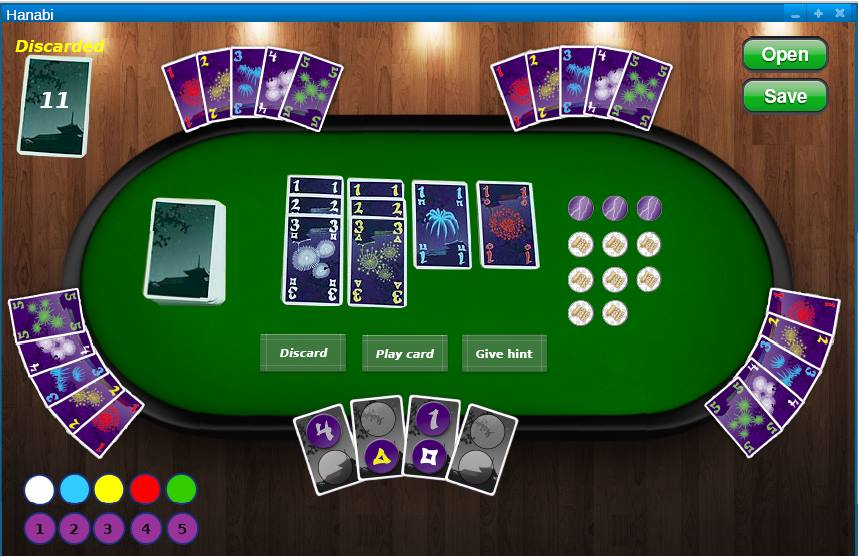
\includegraphics[scale = 0.4]{ihm.jpg}
\caption{Prototype d'interface graphique sur lequel on se base pour notre implémentation.}
\end{figure}

\subsection{Besoins non fonctionnels}

\noindent
L'intelligence artificielle doit décider de son prochain coup en un temps limité afin que la partie se déroule normalement. Il est donc indispensable que les IAs soient efficaces et optimisées. \\

\noindent
Nous avons réfléchi à plusieurs possibilités pour les IAs :\\

\begin{itemize}
    \item[$\bullet$] {\bfseries Une IA simple} : cette IA joue d'une manière basique: elle joue une carte valide si possible (quand elle connaît la carte, et elle peut être posée), sinon, elle donne des indices aléatoires tant que des jetons sont disponibles, dans le cas contraire elle défausse une carte (en priorité les cartes déjà posées ou les cartes sans indices).\\
    \item[$\bullet$] {\bfseries Une IA sans risque} : cette IA ne joue des cartes que quand elle les connaît. Dans le cas contraire, elle évaluera s'il vaut mieux défausser une carte ou de donner un indice et lequel.\\
    \item[$\bullet$] {\bfseries Une IA qui prend des risques} : cette IA est moins adverse au risque. En utilisant une heuristique, elle évalue les probabilité de réussite des différentes actions possible et choisi le meilleur coup. \\
    \item[$\bullet$] {\bfseries Une IA omnisciente} : cette IA connaît toutes les cartes (même les siennes), elle se concentre donc sur les priorités entre les différents coups possibles (jouer une carte qu'on connaît, défausser des cartes pour gagner des jetons <<indice>> ou donner des indices aux autres joueurs) 
\end{itemize}


\subsection{Critères d'acceptabilité du produit}

\noindent
Notre but est de simuler un jeu entre deux ou plusieurs humains, en utilisant des IAs. Nous avons donc besoin d'avoir des intelligences artificielles efficaces qui ne prennent pas trop de temps pour calculer leur prochain coup. Nos critères d'acceptabilité par rapport aux intelligences artificielles sont donc :\\

\begin{itemize}
    \item[$\bullet$] De permettre à l'utilisateur de jouer une partie de Hanabi sans devoir attendre trop longtemps pour son tour.

    \item[$\bullet$] L'intelligence artificielle est considérée comme efficace si elle atteint systématiquement un score entre 20 et 25 (le score maximum possible) en ne jouant qu'entre des IAs avec la même stratégie.\\
\end{itemize}

\noindent
Nous voulons aussi que le jeu soit facile et simple à jouer pour le joueur humain, donc une interface claire et compréhensible est indispensable. Il faut que toute personne soit capable de s'en servir. Nous voulons aussi avoir au moins une IA qui joue de façon réaliste plutôt que d'essayer de faire un score maximal.\\


\section{Analyse et conception}

\subsection{Modélisation exhaustive d'une situation}

\noindent
Ici le but est d'identifier chaque situation de jeu possible par un monde de Kripke.\\

\noindent
La première étape est de modéliser les mondes liés à la main (combinaison de 4 ou 5 cartes sans ordre) du joueur, c'est à dire toutes les mains possibles en prenant en compte les cartes vues, déjà jouées ou déjà défaussés. L'agent correspondant au joueur hésite donc entre tous ces mondes possibles.\\

\noindent
Notre structure de Kripke est donc:\\

$\mu=\{U,\{R_{1}\},I \}  $\\
$   U=\{M_{1},...M_{m} \}   $\\

\noindent
$R$: A ce stade, $R_{1}$ connecte tous les mondes, on suppose que l'on ne génère pas les mondes qu'il sait déjà impossibles.\\

\noindent
$I$: On note    $C_{j,c,v}$ la variable affirmant que le joueur j possède une carte de couleur c et de valeur v. Pour n joueurs, un monde $M_{i}$ contiendra donc toujours un nombre de variables $nv=n*4 | n>3$ ou $nv=n*5 | n<4$\\

\noindent
A ce niveau de modélisation, on peut déjà envisager des prises de décisions probabilistes simplement en comptant le nombre de mondes dans lesquels faire telle action aurait un impact positif.\\

\noindent
Ensuite, il est également possible pour le joueur de modéliser les mondes entre lesquels il pense qu'un autre joueur hésite. Appelons le joueur qui réfléchit $j1$ et celui sur lequel il porte sa réflexion $j2$. Cela pose problème car ce $j2$ dispose d'informations que n'a pas $j1$ (ses propres cartes), mais on peut tout de même savoir que des mondes sont impossibles grâce à l'information commune aux 2 joueurs (les cartes des autres joueurs, les cartes jouées, les cartes défaussées, les indices donnés).
Pour cela, on peut se baser sur les formules de la logique propositionnelle, auxquelles on ajoute la modalité de la connaissance: $[]_j$ Les atomes sont représentés sous la forme :$\Phi_{j,c,c1,v1}$ tels que "la carte $c$ du joueur $j$ a la couleur $c1$ et la valeur $v1$". L'utilisation de l'axiome de connaissance est donc   $[]_j F$ est vrai dans un monde $M$ si tous les $M'$ successeurs de $M$ pour la relation $R_j$ satisfont $F$. Ce raisonnement peut être appliqué pour chaque autre joueur.\\

\noindent
On a donc maintenant:\\

$\mu'=\{U',\{R_{1},...,R_{n}\},I' \} $\\

$U'=\{M_{1},...M_{m'} \} $\\

\noindent
Pour les relations $R_{i}$, il faut se dire que le joueur $i$ n'hésite qu'entre les mondes où toutes les cartes sont identiques sauf les siennes.\\

$   \forall i \in [2,...,n] ,  \forall (M_{j},M_{k}) \in U'*U',$\\

$R_{i}(M_{j},M_{k}) 
\equiv
\forall l \in [1,...,n]|l \ne i,  \forall C_{l,c1,v1} \in  I(M_{j}), \forall C_{l,c2,v2} \in  I(M_{k}), c1=v1, c2=v2    $\\

\noindent
Ensuite, il faut tenir compte des indices donnés par les joueurs qui sont des "annonces publiques" qui viennent enrichir la connaissance commune à tous les joueurs. Grâce à ces annonces et aux formules proposées plus haut, il est possible de supprimer des membres des relations (graphiquement, cela correspond à supprimer des arrêtes du graphe), et donc certains monde deviennent impossibles.


\subsection{Modélisation carte par carte}

\noindent
Cette fois, l'objectif est de créer des structures de Kripke pour chaque carte plutôt que pour chaque situation. Ainsi, sans information, il y aurait 25 mondes pour chaque carte. On peut ensuite tenter d'appliquer les mêmes raisonnements que dans la modélisation exhaustive.\\

Univers de la i-ème carte du joueur $j$:\\

$   \mu_{i,j}=\{U,\{R_{1},...,R_{n}\},I \}  $\\

$   U=\{M_{1},...M_{m} \}   $\\

$I$: chaque monde contient 2 variables, une pour la couleur et une pour la valeur. \\

$\forall M \in U, I(M)=(c,v)|c\in[rouge,bleu,vert,jaune,blanc],v\in[1,...,5]$\\

\noindent
Cette approche peut être utilisée comme la précédente pour choisir les coups à jouer de manière probabiliste. Cependant, si l'on veut essayer de raisonner sur la connaissance des joueurs, il est nécessaire de mettre en relation tous ces univers, et on en revient donc à la modélisation exhaustive. Cette approche n'est donc pas réellement intéressante,puisque il est possible d'utiliser des raisonnement probabilistes sans structures de Kripke. 

\subsection{Situations de jeu interessants - A FAIRE Catalina + Cédric}

\subsection{Intelligences artificielles - A FAIRE}

\noindent
Fonctionnement, évaluation et tests

\subsubsection{DummyIA - A FAIRE Catalina}

\subsubsection{SemiDummyIA - A FAIRE Cédric}

\subsubsection{Heuristique IA - A FAIRE Cédric}

\subsection{Déroulement du projet - A FAIRE Catalina}

\noindent
Comment nous avons avancé le projet.

\subsection{Architecture - A FAIRE Cédric + Daniel}

\noindent
L'architecture de notre code (MVC), etc.

\subsection{Diagrammes de classe - A FAIRE Cédric + Daniel}

\section{Documentation}

\noindent
Le logiciel doit être accompagné d’un document expliquant les règles du jeu, ainsi que d’un manuel d’utilisation. Le code sera accompagné d'une Javadoc pour décrire le fonctionnement de notre code. Il y aura également un rapport sur le déroulement du projet, expliquant en détail les raisonnements utilisés.

\subsection{Cahier des charges - A FAIRE Catalina}

\subsection{Manuel d'utilisation - A FAIRE Catalina}

\section{Tests - A FAIRE Matthieu}

\noindent
Qu'est-ce que vous entendez par rapport aux tests ? (Tests JUnit, le bon fonctionnement de l'interface graphique, tests IA)

\end{document}
